\title{Multilayer Perceptron}
\label{chp:multilayer-perceptron}
\author{Lucas Costa \and Márcio Guerreiro \and Erickson Puchta \and Yara de Souza Tadano \and Thiago Antonini Alves \and  Maurício Kaster \and Hugo Valadares Siqueira}
\authorrunning{Costa et al.}
\institute{UTFPR - Universidade Tecnológica Federal do Paraná}
\maketitle

Artificial Neural Networks (ANNs) are computationally intelligent systems inspired by higher organisms' nervous system behavior. They are based on processing units called artificial neurons, capable of calculating mathematical functions \cite{haykin}. Through these neurons and their connections, ANNs can learn to process information to produce the expected output \cite{Castro2006FundamentalsON}. ANNs can be seen as general tools for solving different problems. Thus, they are often applied in tasks such as pattern classification, data mining, regression/approximation of functions, and information processing, being useful in several areas of knowledge \cite{haykin}.
This chapter will explain the MultiLayer Perceptron (MLP), the best-known ANN architecture.  For that, the concept of artificial neuron, the primary processing structure of an MLP, will first be introduced.


%%%%%%%%%%%%%%%%%%%%%%%%%%%%%%%%%%%%%%%%%%%%%%
\section{Artificial Neuron}
\label{sec:neuronio}

The artificial neuron is inspired by the biological neuron. In biological systems, neural impulses are received through dendrites and processed in the cell body. Depending on the result of the integration of the received signals, if they are higher than a critical threshold, the neuron may or may not produce a new impulse (action potential), which will, in turn, be transmitted to other neurons connected to its axon terminals \cite{Castro2006FundamentalsON}. The axon union with dendrites is called a synapse, which works as a valve controlling the flow of information (impulses) between neurons. The synapse is variable, hence, with the ability to adapt and learn.

Figure \ref{fig:neuronio} shows the generic artificial neuron scheme used in ANNs. This device receives a set of $\textbf{x} = [ x_1 , x_2 ,..., x_I]$ inputs, which may come either from other neurons or correspond to the input variables of the problem. When they correspond to the input variables of the problem, $I=d$ is the dimensionality of the problem. It then processes this information, and responds with a $\hat{y}_j$ signal, where $j$ the current neuron. This response, which is a transformation of the received inputs, is either propagated to other neurons or given as the output of the ANN.

\begin{figure}[h!]
	\begin{center}
		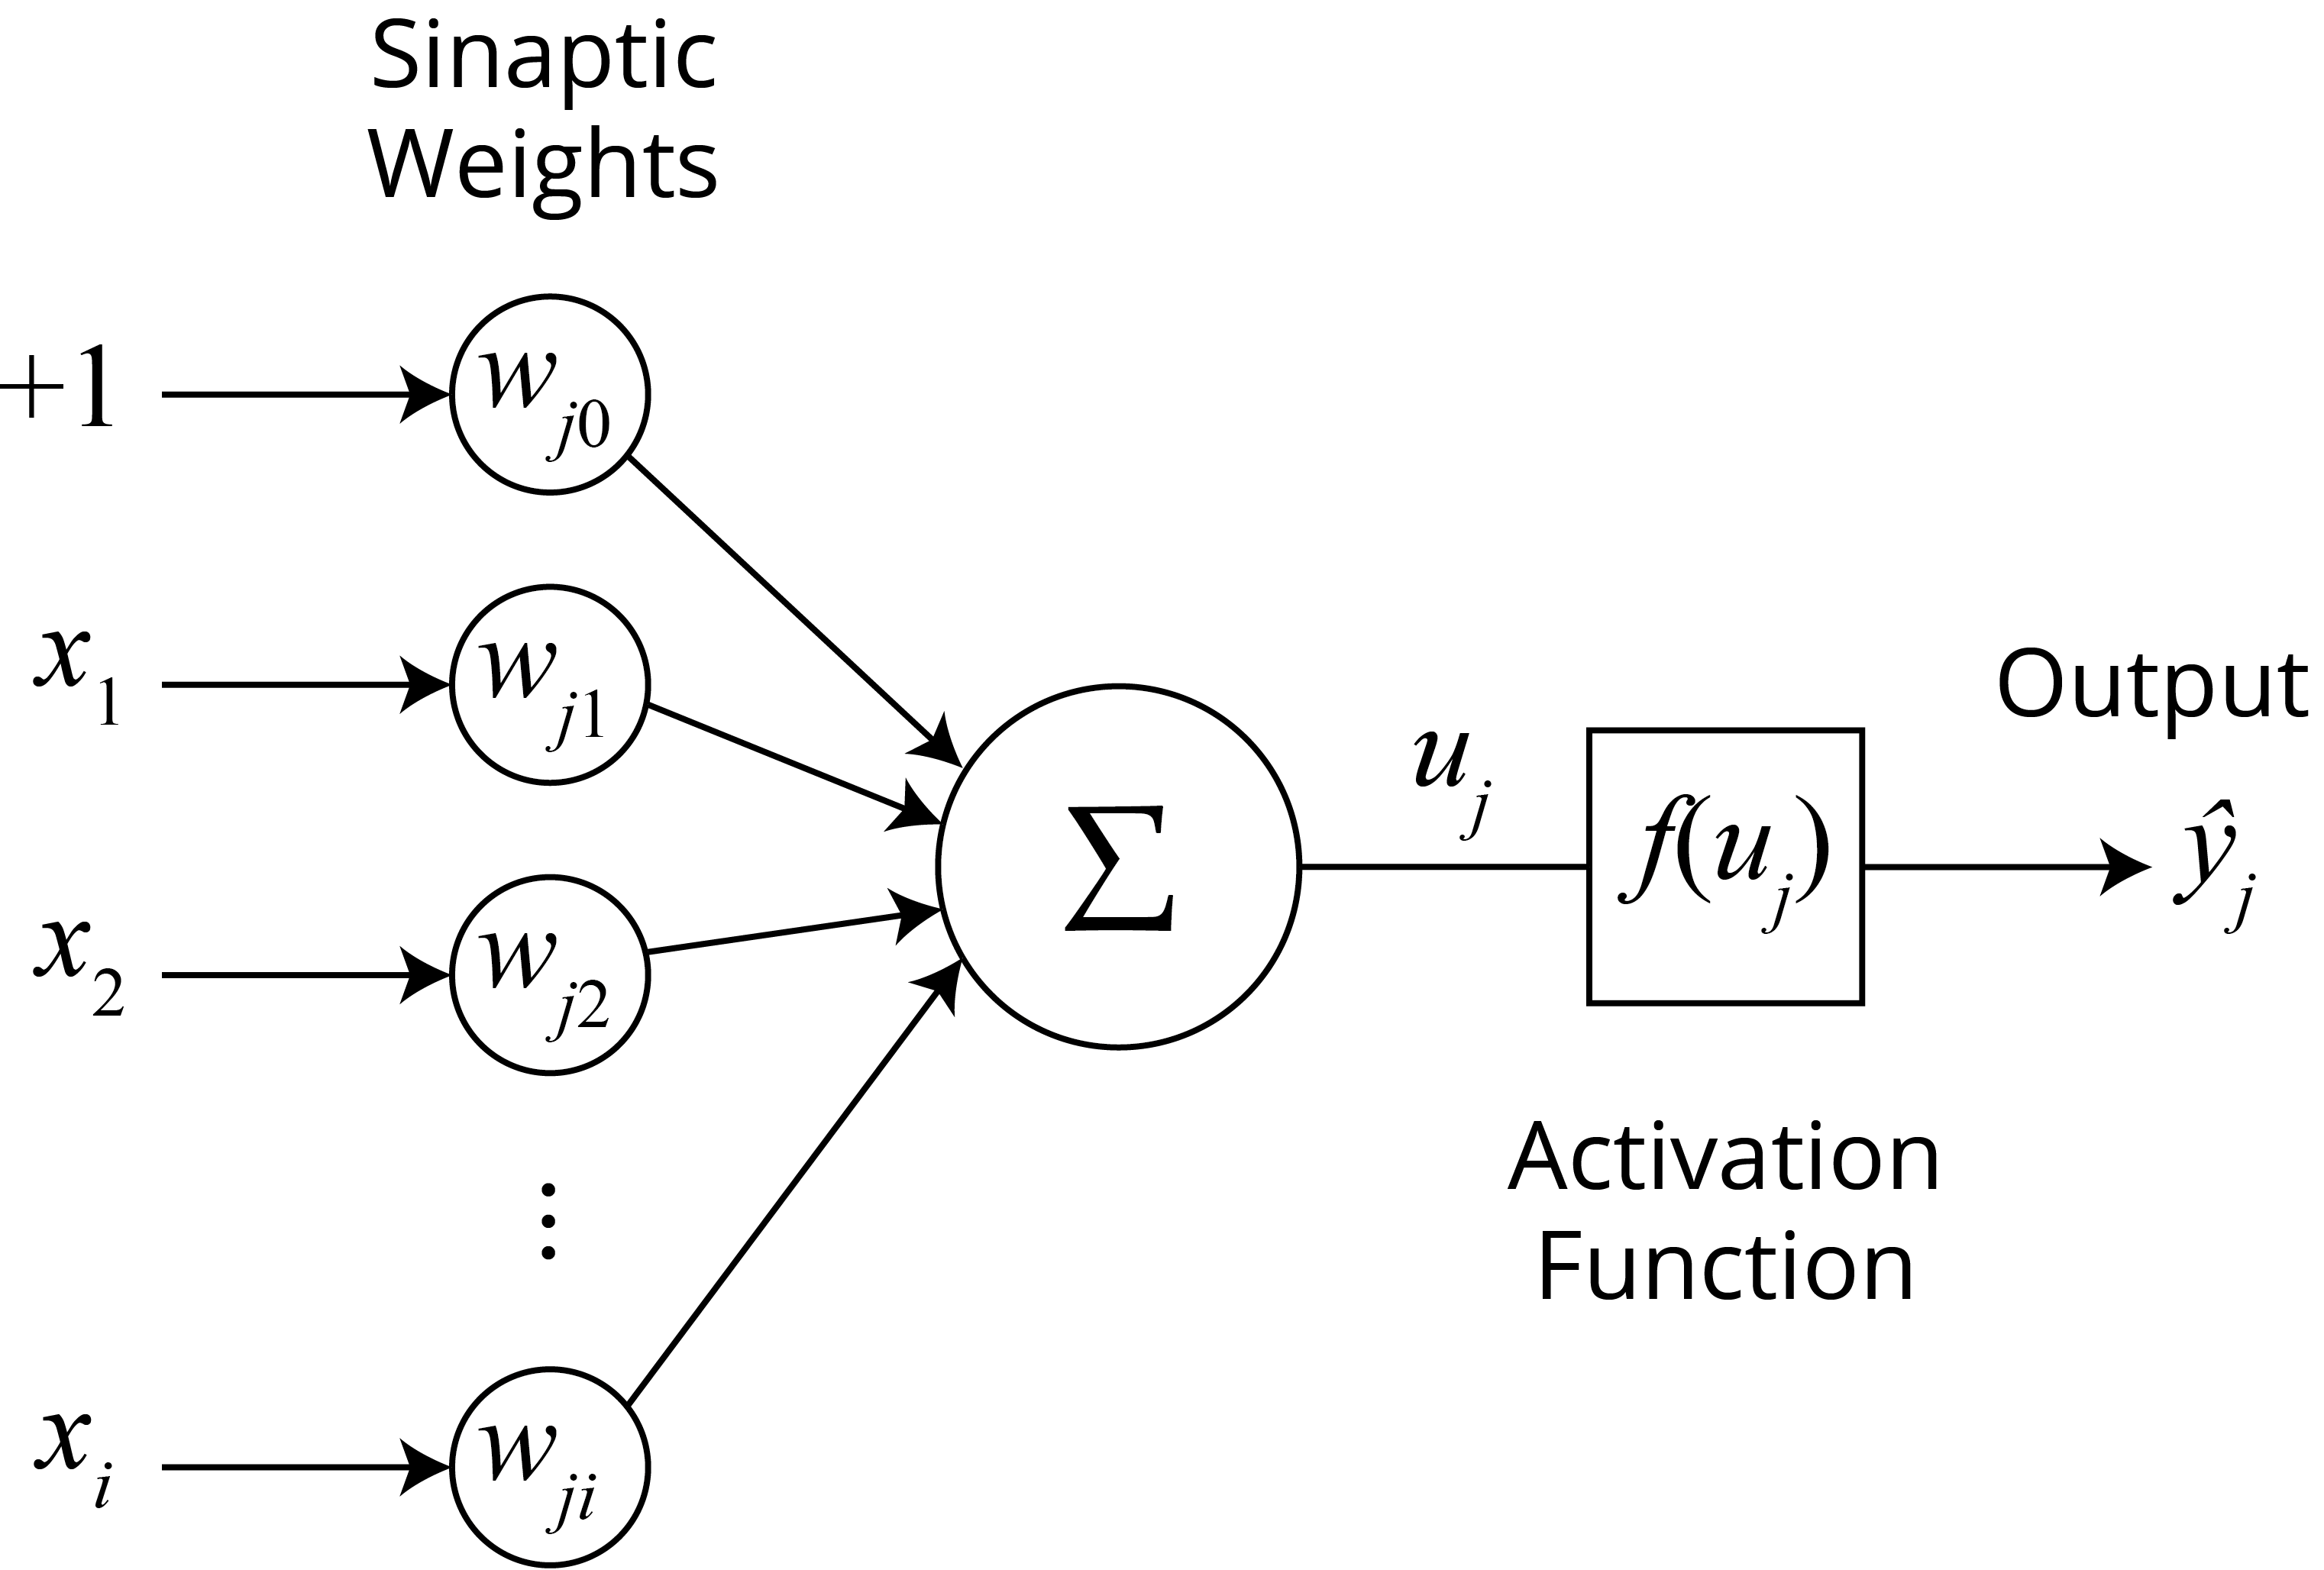
\includegraphics[width=0.8\textwidth]{"Part 3 - Learning Systems/Supervised Learning/Multilayer Perceptron/figures/neuronioArtificial_v2@4x.png"}
	\end{center}
	\caption{Scheme of an artificial neuron.}
	\label{fig:neuronio}
\end{figure}

The processing performed by neuron $j$ consists in weighting the input signals $x_i , i=1, 2,..., I$ and a fixed value bias signal $x_0=+1$ by the weights $w_{ji}$ of this neuron. Then, the sum of the weighted input signals $u_j$ (a.k.a. activation value) passes through an activation function $f(\cdot)$, generating the output $\hat{y}_j$. The mathematical representation of this model is given by Equation \ref{eq:neuronio}:


\begin{equation}
    \label{eq:neuronio}
    \hat{y}_j = f(u_j) = f \left( \sum_{i=0}^I w_{ji} x_i  \right).
\end{equation}

%%%%%%%%%%%%%%%%%%%%%%%%%%%%%%%%%%%%%%%%%%%%%%%
%\subsection{Activation Functions}
\label{ssec:ativacao}

An activation function $f(\cdot)$ defines the output of a given neuron, given the activation value $u$. Several functions have already been used or developed. This section gives some examples of such functions.

The linear activation function is a simple function that can be described by equation \ref{eq:funcaoAtivacaoLinear}: 

\begin{equation}
	\label{eq:funcaoAtivacaoLinear}
	f(u) = \alpha u,
\end{equation}
where $\alpha$ is a real number.

Another standard function is the signal, also known as \textit{Heaviside} \cite{haykin}, which can respond in a binary $\{0, 1\}$ or bipolar $\{-1, 1\}$ way. The former is the one used in the McCulloch and Pitts neuron \cite{McCulloch1990}, as shown in Equation \ref{eq:funcaoAtivacaoMCP}:

\begin{equation}
	\label{eq:funcaoAtivacaoMCP}
	f(u) = \left\{\begin{matrix}
		0, & u \leq 0    \\
		1, & u > 0 \: .
	\end{matrix}\right.
\end{equation}

A group of functions most commonly used in the hidden layers of an MLP are the sigmoid functions \cite{haykin, Castro2006FundamentalsON}. Their plot has the peculiar shape of an ``S". They represent a balance between linear and nonlinear behavior, which can be obtained from several functions, such as the logistic function and the hyperbolic tangent \cite{Jeffrey2008}. The logistic function is defined by Equation \ref{eq:funcaoAtivacaoLogistica}:

\begin{equation}
	\label{eq:funcaoAtivacaoLogistica}
	f(u) = \frac{1}{1 + e^{-u}}\:.
\end{equation}

The hyperbolic tangent is defined by Equation \ref{eq:funcaoAtivacaotanh}:

\begin{equation}
\label{eq:funcaoAtivacaotanh}
	f(u) = \frac{e^u - e^{-u}}{e^u + e^{u}}\:.
\end{equation}

The wide use of S-Shaped functions is also due to some key features \cite{Menon1996}:

\begin{itemize}
    \item This kind of function is continuous and differentiable at all points, allowing learning with popular derivative-based learning algorithms such as gradient descent;
    \item They have output saturation, which can prevent the output signal of each neuron from diverging;
    \item It is possible to use them to create different mappings since these functions have an almost linear character in the region around the origin, while tt the same time, close to saturation, they are strongly nonlinear.
\end{itemize}

Recently, with the advancement of ANNs studies and, more specifically, \textit{deep learning} methods, new activation functions have been developed to solve vanishing gradients or flat surfaces \cite{Fahlman1988}, which are problems that learning algorithms such as gradient descent may face and that may prevent them from being able to successfully learn the weights of the neurons.

One new activation function, the Rectified Linear Unit or ReLU \cite{Maas2013}, can be expressed by Equation \ref{eq:relu}:
\begin{equation}
	\label{eq:relu}
	f(u) = \left\{\begin{matrix}
		u, & u > 0    \\
		0, & u \leq 0 \:.
	\end{matrix}\right.
\end{equation}

\noindent
If $u$ is greater than zero, the output will equal the input. So, the ReLU function is similar to the linear activation function (Equation \ref{eq:funcaoAtivacaoLinear}) for values greater than zero. %, com exceção da presença de um número real $\alpha$. 

Another newly developed function is the Exponential Linear Unit or ELU \cite{Clevert2016}. Its definition is expressed by Equation \ref{eq:relu}:

\begin{equation}
	\label{eq:elu}
	f(u) = \left\{\begin{matrix}
		u,               & u > 0    \\
		\alpha(e^u - 1), & u \leq 0 \:,
	\end{matrix}\right.
\end{equation}

The definition for $u$ lower than zero allows problems with negative values.

%%%%%%%%%%%%%%%%%%%%%%%%%%%%%%%%%%%%%%%%%%%%%%%%%%%%%%%%%%
\section{MLP Architecture}
\label{sec:mlp}

One of the best-known ANN architectures is the MultiLayer Perceptron (MLP), which structurally generalizes the artificial neuron called Rosenblatt perceptron \cite{Rosenblatt1958} -- an artificial neuron that uses the Heaviside activation function. As demonstrated by \cite{Cybenko1989}, this ANN has universal approximation capability: an MLP can approximate any continuous, bounded, differentiable, nonlinear function with defined inputs in a compact space with arbitrary precision. This is possible by the additive composition of base functions, which, for MLP, are ridge functions. However, this theorem does not specify the amount of artificial neurons required, nor does it define any method for adjusting the value of the weights so that the optimal configuration of the network is guaranteed.

MLPs organize neurons in several layers chained together, where each layer is the arrangement of parallel neurons. Neurons in a given layer do not communicate with each other, and only send their output signals forward, which is known as a \textit{feedforward} structure. MLPs contain an input layer, one or more hidden layers and an output layer. Figure \ref{fig:mlp} shows an example of possible MLP structure with one hidden layer for a problem with $d$-dimensional input variables and one output variable. As the neurons are organised in layers, we use superscript numbers in our notation to identify their layer. The first layer ($l=0$) is the input layer, whose neurons receive as inputs the input variables of the problem. Each neuron in this layer is a special neuron that simply feeds the value of a given input feature to the nodes in the hidden layer, i.e., $\hat{y}^{(l=0)}_j = x_j$, where $j$. Neurons in the hidden layers ($0<l<L$) and output layer ($l=L$) are standard artificial neurons that receive as inputs the outputs of the neurons from the previous layer. The last layer is the output layer, whose neurons produce the values of the output variables of the problem. 

One or more hidden layers can be used.  The hidden layers are responsible for mapping the input signal in a nonlinear way into another space, according to the demand of the problem. As the combination of linear functions is also a linear function, the activation functions of the hidden nodes is usually not a linear function. 

When dealing with regression or binary classification problems, a single output node is typically used. When dealing with multi-class classification problems, one output node is used to correspond to each class. After the training process of the MLP is complete, predictions are given by mapping the numeric values given by the output nodes into classes when dealing with classification problems. In particular, sigmoid logistic activations are typically used in the output node for binary classification problems. If the output value is larger than 0.5, a given class could be predicted. If the output value is smaller than or equal to 0.5, the other class could be predicted.  


\begin{figure}[h!]
    \centering
    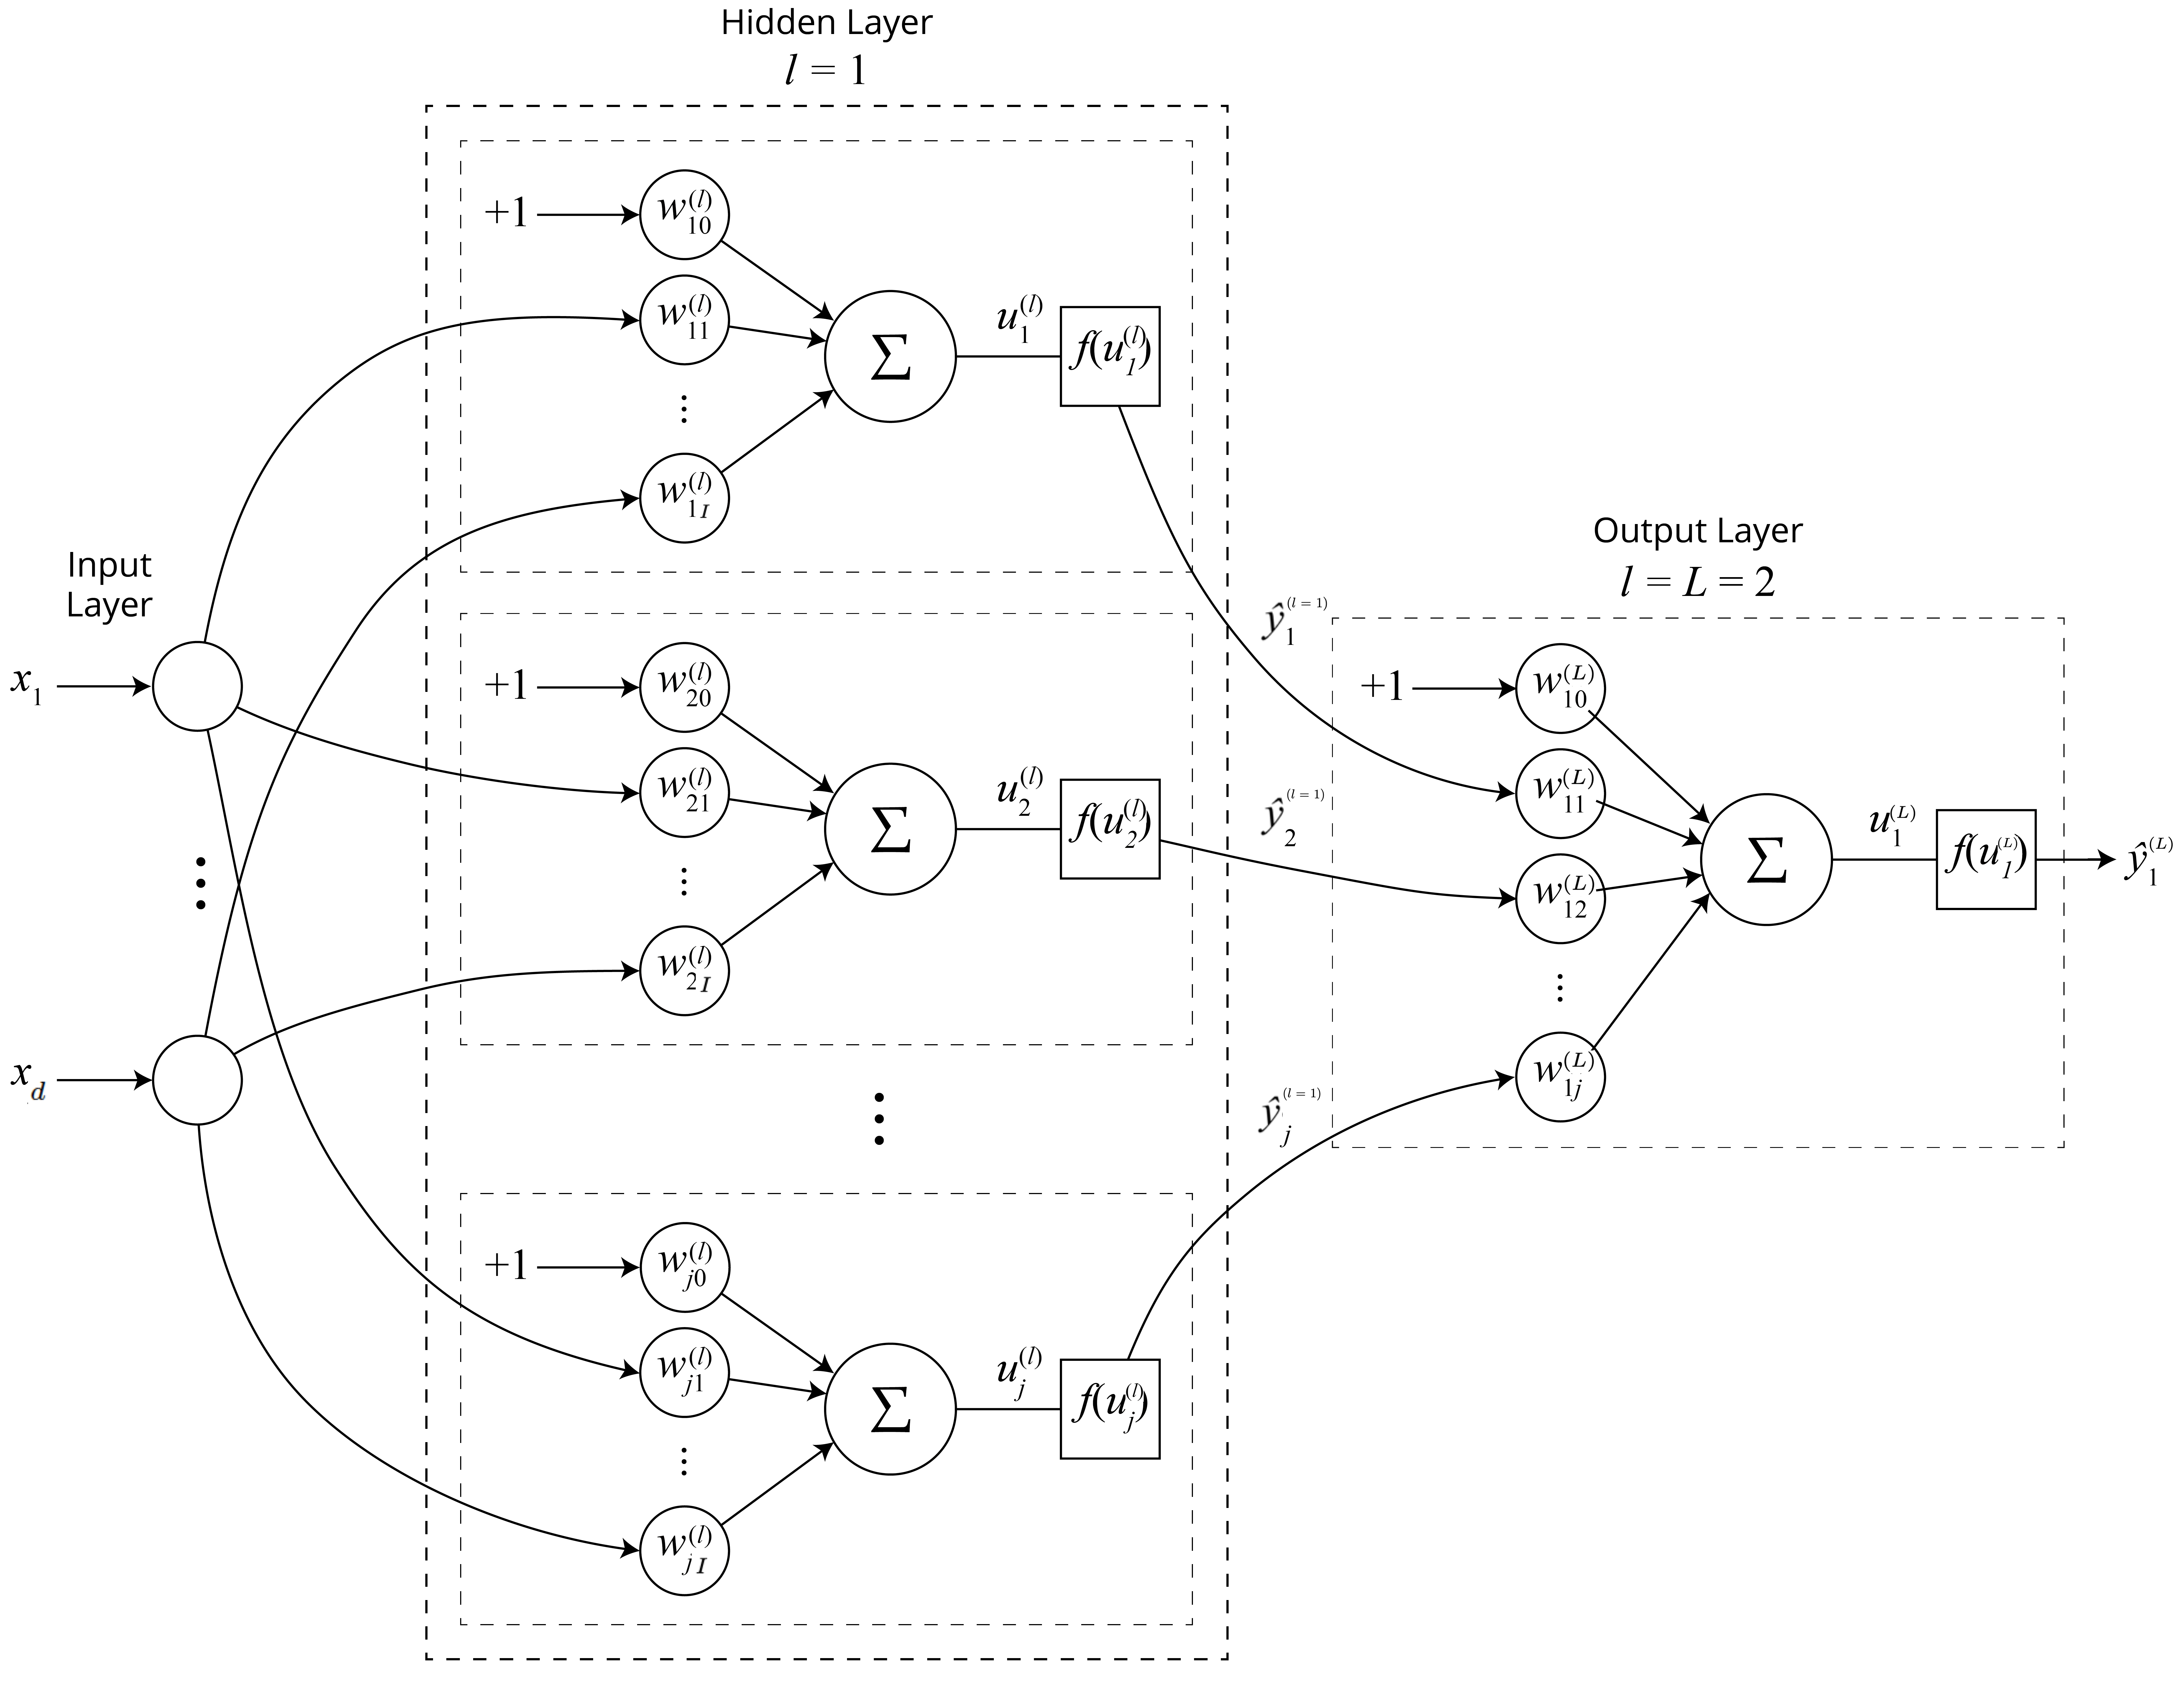
\includegraphics[width=1\textwidth]{"Part 3 - Learning Systems/Supervised Learning/Multilayer Perceptron/figures/MLP_v2@4x.png"}
    \caption{Example of MLP.}
    \label{fig:mlp}
\end{figure}





%%%%%%%%%%%%%%%%%%%%%%%%%%%%%%%%%%%%%%%%%%%%%%%%%%%%%%%%%%%%
\section{Training}
\label{ssec:treino}

Several training algorithms are aimed at adjusting the weights of an MLP. For that reason, the weights of the MLP are also referred to as ``parameters'' to be learned by the training process. This chapter will focus on the traditional gradient descent method with the famous backpropagation algorithm \cite{rumelhart1986learning}.

The training process of an MLP is typically supervised, relying on a training set containing labelled training examples with the values of the input variables and the corresponding desired values of the output variables. When using backpropagation, training consists of two steps: forward and backward. In the forward step, the network weights do not change; they are fixed, and the input data (from the training set) is propagated from the first to the last layer to obtain the network output. Then, an error signal is produced by comparing the obtained output with the desired one. After that, the gradient vector of the error function is calculated. Based on it, the backward step applies the gradient descent optimization method from the last to the first layer, such that the weights of the neurons are adjusted in the opposite direction of the gradient, i.e., in the ``steepest descent'' direction that most decreases the error function \cite{haykin}. The forward and backward propagation of the whole training set are applied iteratively until some sopping criterion is reached \cite{Castro2006FundamentalsON}. Each iteration through the whole training set is typically referred to as an epoch. The most used error function for this task is the Mean Squared Error (MSE).  In Section \ref{ssec:Pseudocodigo}, this procedure is presented in a mathematical format. 

It is worth noting that this procedure is nothing more than an optimization algorithm being applied to an unconstrained nonlinear optimization problem. Even though this chapter describes the use of gradient descent to optimize the weights, any unconstrained nonlinear optimization method of 1st or 2nd orders could be used, such as the gradient and Levenberg-Marquardt methods. Note that such a premise is not based on biological inspiration.

There are different learning methods to handle the adjustment of network weights based on gradient descent \cite{haykin, Bengio2012}:

\begin{itemize}
	\item Batch learning: weight adjustments occur after all training examples are presented to the network, at the end of each epoch during the training;
	\item Online learning: weight adjustments occur after the presentation of each training example, turning the search for optimal weights into a stochastic search since the examples are presented in random order;
	\item Mini-batch learning: this an intermediate process between batch and online learning, where weight updates are performed after fixed size batches of examples from the training set are presented.
\end{itemize}

%%%%%%%%%%%%%%%%%%%%%%%%%%%%%%%%%%%%%%%%%%%%%%%%%%%%%%%%%%%%
\subsection{Backpropagation}
\label{ssec:Pseudocodigo}

This section follows the definitions of Simon Haykin \cite{haykin} to formalize the backpropagation algorithm. The online learning version of Backpropagation is presented.

Before starting the learning process, the weights of the MLP are typically initialized uniformly at random in the interval $[-1,+1]$. If there is some previous knowledge about the mapping process being worked on, it is possible to initialize the weights with pre-fixed values.  

The first step in applying Backpropagation is the propagation of the input signal passing through the input and hidden layers until reaching the output layer (forward step). 
Consider a given training example ($\mathbf{x}(n), \mathbf{y}(n)$) being introduced in a given iteration $n$, where $\mathbf{x}(n)$ are the input variables fed to the ANN input layer, and $\mathbf{y}(n)$ is the desired output. The input layer simply feeds the values of the input features to the hidden layer. From the hidden layer to the output layer, the input values propagation is done by calculating the $u_j^{(l)}(n)$  induced by neuron $j$ in layer $l$ (Equation \ref{eq:backprop1}):


\begin{equation}
\label{eq:backprop1}
    u_j^{(l)}(n) = \sum_i w_{ji}^{(l)}(n) \hat{y}_i^{(l-1)}(n),
\end{equation}
where the value $w_{ji}^{(l)}(n)$ is the weight connecting neuron $j$ of layer $l$ to neuron $i$ from layer $l-1$, and
$\hat{y}_i^{(l-1)}(n)$ is an input of neuron $j$ of layer $l$ corresponding to the output signal of neuron $i$ of the previous layer $l-1$ (or the bias value +1, if $i=0$).

The output of neuron $j$ from layer $l$ can be defined by Equation \ref{eq:backprop2}:

\begin{equation}
\label{eq:backprop2}
    \hat{y}_j^{(l)}(n) = f_j (u_j^{(l)} (n) ),
\end{equation}

If the neuron $j$ is in the first hidden layer ($l = 1$), then Equation \ref{eq:backprop3} is used:

\begin{equation}
    \label{eq:backprop3}
    \hat{y}_j^{(0)}(n) = x_j (n),
\end{equation}
where $x_j(n)$ is the $j$th element of the input vector $\mathbf{x}(n)$. 

%However, if the neuron $j$ is in the output layer ($l = L$), where $L$ equals the total number of layers of the network, then Equation \ref{eq:backprop4} is used:
%
%\begin{equation}
%    \label{eq:backprop4}
%    \hat{y}_j^{(L)} = o_j (n).
%\end{equation}

The second step of the backpropagation (backward) is then performed to propagate the error backward through the MLP, using it to adjust the weights based on gradient descent. The error for each neuron in the output layer is calculated according to Equation \ref{eq:backprop5}: 

\begin{equation}
    \label{eq:backprop5}
    e_j (n) = \hat{y}^{(L)}_j(n) - y_j (n),
\end{equation}
where $y_j (n)$ is the $j$th output of the desired output vector $\mathbf{y}(n)$.

Afterwards, the local gradients $\delta$ of the network are calculated. The local gradient of the output layer $L$ is obtained by Equation \ref{eq:backprop6}:

\begin{equation}
    \label{eq:backprop6}
    \delta_j^{(L)} (n) = e_j(n) {f}'_j (u_j^{(L)}(n)),
\end{equation}
and those of the other layers are following Equation \ref{eq:backprop7}:

\begin{equation}
    \label{eq:backprop7}
    \delta_j^{(l)} (n) = {f}'_j (u_j^{(l)}(n)) \sum_k \delta_k^{(l+1)} (n) w_{kj}^{(l+1)}(n),
\end{equation}
where ${f}'_j(\cdot)$ is the derivative of the activation with respect to the activation value.

Finally, the adjustment of the weights of the layer $l$ takes place according to the generalized delta rule of Equation \ref{eq:backprop8}:

\begin{equation}
    \label{eq:backprop8}
    w_{ji}^{(l)} (n+1) = w_{ji}^{(l)}(n) + \eta \delta_j^{(l)}(n) \hat{y}_i^{(l-1)} (n).
\end{equation}

One way to improve the weight adjustment process and avoid instabilities is to modify Equation \ref{eq:backprop8} by adding a term called \textit{momentum}, changing Equation \ref{eq:backprop8} to Equation \ref{eq:backprop9}:

\begin{equation}
\label{eq:backprop9}
    w_{ji}^{(l)} (n+1) = w_{ji}^{(l)}(n) + \alpha[\Delta w_{ji}^{(l)}(n-1)] + \eta \delta_j^{(l)}(n) \hat{y}_i^{(l-1)} (n),
\end{equation}
where $\alpha$ is a generally positive constant and $\Delta w_{ji}^{(l)}(n) = w_{ji}^{(l)}(n) - w_{ji}^{(l)}(n-1)$. The momentum term can reduce instability in the weights by enabling the previous change in the weight to influence the current change.

The forward and backward steps are repeated, presenting all training data again until some stopping criterion is reached. Backpropagation with gradient descent can be summarized in Algorithm \ref{alg:backprop}.

%%%%%%%%%%%%%%%%%%%%%%%%%%%%%%%%%%%%%%%%%%%%%%%%%%%%%%%%%%%%

\begin{algorithm}[h!]
    \caption{Backpropagation. \label{alg:backprop}}
    
    Parameters: max\_it, $\eta$, $\alpha$, $\mathcal{T}$
    
    Output: $\mathbf{w}$
    
    \begin{algorithmic}[1] 
        \STATE Initialize $\mathbf{w}(1)$
        \STATE n $\leftarrow 1$
        \STATE epoch $\leftarrow 1$

        \WHILE{epoch $<$ max\_it}
		\STATE Shuffle the order of the training data in $\mathcal{T}$
		\FOR{each example in $\mathcal{T}$}
			\STATE Refer to this example as $\mathbf{x}(n),\mathbf{y}(n)$ 
            \FOR{$l$ from $1$ to $L$}
                
                \FOR{each neuron $j$ in layer $l$}
                    \FOR{each input $i$ of neuron $j$}
                        %\STATE $u_j^{(l)}(n) \leftarrow u_j^{(l)}(n) + w_{ji}^{(l)}(n) \hat{y}_i^{(l-1)}(n)$ \COMMENT{Equation \ref{eq:backprop1}}
                        \STATE $u_j^{(l)}(n) = \sum_i w_{ji}^{(l)}(n) \hat{y}_i^{(l-1)}(n)$ \COMMENT{Equation \ref{eq:backprop1}}
                    \ENDFOR

					
                \ENDFOR
            
            \ENDFOR
            

            \FOR{each neuron $j$ of layer $L$}
                    \STATE $e_j (n) \leftarrow \hat{y}_j(n)^{(L)} - y_j (n)$ \COMMENT{Equation \ref{eq:backprop5}}
            \ENDFOR


            \FOR{$l$ from $L$ down to $1$}
                \FOR{each neuron $j$ in layer $l$}
                    \IF{$ l = L $}
                        \STATE $ \delta_j^{(L)} (n) \leftarrow e_j(n) {f}'_j (u_j^{(L)}(n)) $ \COMMENT{Equation \ref{eq:backprop6}}
                    \ELSE
                    	  \STATE $\delta_j^{(l)} (n) \leftarrow 0$
                        \FOR{each neuron $k$ in layer $l+1$}
                            \STATE $ \delta_j^{(l)} (n) \leftarrow \delta_j^{(l)} (n) + {f}'_j (u_j^{(l)}(n)) \delta_k^{(l+1)} (n) w_{kj}^{(l+1)}(n) $ \COMMENT{Equation \ref{eq:backprop7}}
                        \ENDFOR
                    \ENDIF

                    \FOR{each input $i$ of neuron $j$}
                        \STATE $w_{ji}^{(l)} (n+1) = w_{ji}^{(l)}(n) + \alpha[\Delta w_{ji}^{(l)}(n-1)] + \eta \delta_j^{(l)}(n) \hat{y}_i^{(l-1)} (n)$ \COMMENT{Equation \ref{eq:backprop9}}
                    \ENDFOR
                \ENDFOR

            \ENDFOR

            \STATE $n \leftarrow n + 1 $
		\ENDFOR
            \STATE epoch $\leftarrow$ epoch + 1
        \ENDWHILE
    \end{algorithmic}
\end{algorithm}

%%%%%%%%%%%%%%%%%%%%%%%%%%%%%%%%%%%%%%%%%%%%%%%%%%%%%%%%%%%%%%%%%%%%%%%%%%%

The algorithm receives the learning rate $\eta$, the momentum constant $\alpha$, the training data stored in the set $\mathcal{T}$, and a ``max\_it" variable, which is the stopping criterion of the algorithm. The training stops when it reaches the defined number of iterations. The MLP's weights are then returned. Another common stopping criterion would be to calculate the error at the end of each iteration and check if it is at an acceptable level: if so, the training is stopped. Finally, note that it is necessary to define the number of artificial neurons in the hidden layer a priori.

%%%%%%%%%%%%%%%%%%%%%%%%%%%%%%%%%%%%%%%%%%%%%%%%%%%%%%%%%%%%%%%%%%%%%%%%%%%
\subsection{Pratical Aspects of the Backpropagation Application}
\label{ssec:Pratical}

The goal of training ANNs is to reach a level of generalization such that it is possible to make correct inferences about data the system does not know. However, the ANN may not perform well with new and unknown data (test set), which were not used during the training phase, characterizing the overfitting phenomenon.

Then, the network's response quality needs to be evaluated during the learning process. A standard procedure separates the available data into three sets: training, validation, and test. As stated, the training set is used to adjust ANN weights. After changing the weights at the end of each training period, the network uses the validation set, which has data not used in training and calculates the output error for this set, keeping the weights fixed. The validation error tends to decrease over the iterations and reach an inflection point when it rises. Thus, an optimal weights array must be saved and overwritten whenever the validation error is reduced during the iterations. When reaching the stopping criterion, the final set of weights of the network will be those saved in the optimal weights array.

The above process is known as cross-validation holdout. Variations can be found in the literature, such as K-fold and leave-one-out \cite{haykin, Castro2006FundamentalsON}. Furthermore, varying the number of neurons (topology) in the hidden layers and comparing the error achieved in the validation set is a strategy to define the number of neurons \cite{James2013}.

A test set whose data were separated from the entire training and validation process is used to assess the final performance of the model. The test set error is expected to be a percentage higher than the training error, although it needs to be an acceptable value. It is a way to measure overfitting even after cross-validating, which is desirable. 

Note that the three sets must be meaningful, containing examples that cover all subspaces that were covered in the original data set. There is no rule for dividing the samples, but the literature frequently uses 70\% for training, 15\% for validation, and 15\% for test. Another possibility is 50\%, 25\%, and 25\%, respectively \cite{haykin}.

It is known that the error-based cost function is multimodal (having multiple minima) for real problems and training algorithms are essentially local optimizers. As mentioned, generating the network weights randomly, respecting a uniform distribution in the interval $[-1,+1]$, is the most common way to initialise the neural network. In this way, initializing the weights to different values leads to different weights being learned. As different learned weights can lead to different training and validation errors, the procedure used to evaluate an ANN approach usually runs it several times (typically at least 30 times), so that the dispersion of results can be evaluated \cite{demvsar2006statistical}. 

Finally, normalizing the data so that they are in the range of the nonlinearity of the activation function is recommended. For example, the data should be normalized over the interval $[0,+1]$ when using the sigmoid function. Similarly, if a hyperbolic tangent option is used, the desired range is $[-1,+1]$. If we deal with a nonlinear mapping or prediction problem, the normalization needs to be reversed, changing the final results to the original data magnitude.

%%%%%%%%%%%%%%%%%%%%%%%%%%%%%%%%%%%%%%%%%%%%%%%%%%%%%%%%%%%%%%%%%%%%%%%%%%%
\section{Exercises}
\label{ssec:exercises}

\begin{enumerate}
\item The truth table for the OR logic gate is shown below:

\begin{center}
\begin{tabular}{cc|c}
\hline
\multicolumn{2}{c|}{Inputs} & \multicolumn{1}{c}{Outputs}                                  \\ \hline
$x_1$         & $x_2$        & $y_{\textrm{OR}}$  \\ \hline
0             & 0            & 0                   \\
1             & 0            & 1                   \\
0             & 1            & 1                  \\
1             & 1            & 1                  \\ \hline
\end{tabular}
\end{center}


For each gate, one could consider a system with desired inputs and outputs. Assume that the inputs are numeric, but treat the output values 0 and 1 as categorical values. Manually create an MLP, including the values of its weights, that is able to perform the OR operation.

%%%%%%%%%%%%%%%%%%%%%%%%%%%%%%%%%%%%%%%%%%%%%%%%%%%%%%%%%%%%%%%%%%%%%%%%%%%%%%%%%
\item  Haberman's Survival Data Set contains cases from a study conducted at the University of Chicago Billings Hospital between 1958 and 1970 on the survival of patients undergoing surgery to treat breast cancer. The attributes are:
\begin{enumerate}
    \item Age of the patient when the procedure was performed;
	\item Year the process took place;
	\item Number of positive nodules detected;
	\item Survivor status, where 1 means the patient survived for five years or more, and 2 represents the patient died before completing five years of surgery.
\end{enumerate}

This database is one of several available ones from the UCI Machine Learning Repository \cite{Dua:2019}. Use the first three attributes as input data for training and the last one as the desired output (surviving or not). Train an MLP and discuss its performance. Vary the number of epochs, hidden nodes, learning rate and momentum, and discuss the impact of that on the results. You may use any existing software to run the MLP. For instance, you may try WEKA: \url{https://www.cs.waikato.ac.nz/ml/weka/}.
\end{enumerate}

%%%%%%%%%%%%%%%%%%%%%%%%%%%%%%%%%%%%%%%%%%%%%%%%%%%%%%%%%%%%%%%%%%%%%%%%%%%%%%%%%
\section{Exercise Answers}

\begin{enumerate}
\item There are many possible answers to this question. One could use an MLP with a single hidden neuron using a sigmoid logistic activation function, with weight of 2 for each of the inputs and weight of -1 for the bias. Interestingly, as this problem is very simple, the hidden node would suffice for providing predictions, without the need for any output node. However, as an MLP should have both a hidden and output layer, we could have a single output neuron using a linear activation function with a weight of 0 for the bias, a weight of 1 for the output of the hidden node, and $\alpha=1$. Such neuron would simply map the output of the hidden node to the output of the MLP.

\item This is a very open question. Please try it out to see how well different configurations of the MLP can perform!
\end{enumerate}

\bibliographystyle{unsrt}
\bibliography{bibliography}
